% !TEX root = _individual/implementation.tex

%%%%%%%%%%%%%%%%%%%%%%%%%%%%%%%%%%%%%%%%%%%%%%%%%%%%%%%%%%%%%%%%%%%%%%%%%%%%%%%%
\chapter{Low-order Discretization Schemes} \label{chap:implementation}

Tensor diffusion---the diffusion of particles through anisotropic media---has
many applications outside of radiation transport, including the fields of geology,
magnetohydrodynamics, and image reconstruction. Numerous tensor diffusion
schemes have been developed, but many of these are more general than is needed
in our work. The anisotropic diffusion tensor derived in
Chapter~\ref{chap:adDerivation} is relatively well behaved: it is a smooth
function in space, it tends toward isotropy in optically thick problems, it is
SPD, and it is diagonally dominant. Additionally, our test problems
are executed in a structured
two-dimensional Cartesian ``brick'' mesh, a simple testbed environment in which
all cells are
quadrilaterals, each interior cell is connected to four adjacent cells through
four faces, and each face is
perpendicular to one of the coordinate system axes.

Because of these simplifying properties, we need not use the more
complex discretization schemes, which have more unknowns
per spatial cell and are therefore more costly to solve.
(An example is the Support Operators Method \cite{Mor1998,Run2006}, with
roughly three unknowns per cell.) Instead, we derive some simple, second-order,
conservative
difference schemes for anisotropic diffusion. Because the
boundary conditions for our AD method are distinct from standard diffusion
boundary conditions, we also present a second-order-accurate discretization of
these.

The ``Anisotropic \Pone'' scheme is entirely new, so we develop a discretization
scheme for it by making a minor modification to the traditional \Pone\
discretization. It uses a ``staggered mesh,'' in which the scalar intensity
$\phi$ is cell-centered and the exiting radiation flux $\vec{F}\vd \vec{n}$ is
edge-centered \cite{War2003}.
% This approach conserves radiation energy, but it does not conserve radiation
% momentum, an important quantity when coupling with hydrodynamics codes
% \cite{Pom1973}.

Each discretization derived in this chapter simplifies to the standard
five-point finite difference diffusion scheme in the case of an
\emph{isotropic} diffusion tensor and a steady-state problem. We admit the
possibility that, because of the simplicity of these discretizations, they were
developed independently decades ago, but an extensive literature search did not
unearth any previously formulated schemes equivalent to ours.

%%%%%%%%%%%%%%%%%%%%%%%%%%%%%%%%%%%%%%%%%%%%%%%%%%%%%%%%%%%%%%%%%%%%%%%%%%%%%%%%
\section{Introduction}

Because the semi-implicit gray TRT formulation of the particle conservation
equation can be expressed as a steady-state transport equation (see
\S\ref{sec:bgSemiImplicit}), for the sake of simplicity we will present the
anisotropic diffusion discretizations without time dependence.

\subsection{Conservation equation}

The steady-state particle conservation equation is
\begin{equation}\label{eq:ssConservation}
  \grad \vd \vec{F}(\vec{x}) + \sigma_a(\vec{x}) \phi(\vec{x}) =
  Q(\vec{x})\,,\qquad \vec{x} \in V\,.
\end{equation}
(In an implicitly discretized time-dependent problem,
$\vec{F}=\vec{F}(t^{n+1})$, $\phi=\phi(t^{n+1})$, $\sigma_a$ is 
the absorption opacity plus the constant $\frac{1}{c\Delta_t}$, and the source
$Q$ contains an additional $\frac{\phi(t^{n})}{c\Delta_t}$.) 

The first step in deriving our finite difference schemes is to assume that the
unknown---%
in this case, $\phi$---is constant over a single cell, represented in
Fig.~\ref{fig:cellDiagram}. 
%
\begin{figure}[tb]
  \centering
  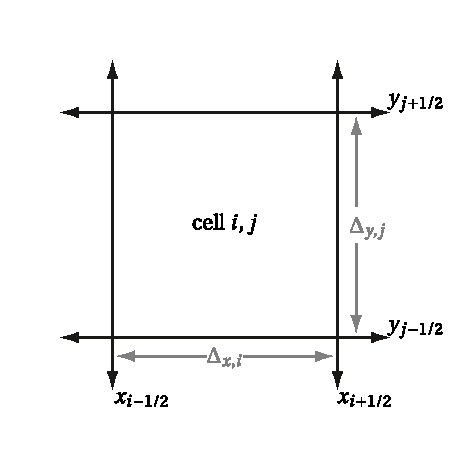
\includegraphics{cell-diagram}
  \caption{Diagram of cell $i,j$.}
  \label{fig:cellDiagram}
\end{figure}
%
We also assume that the effective absorption opacity $\sigma_a$ and source $Q$
are
constant over the cell, which in TRT problems  means approximating the material
temperature as constant over a cell. Integrating Eq.~\eqref{eq:ssConservation} over cell
$i,j$ and applying the divergence theorem gives the following equation:
\begin{equation} \label{eq:ssConservationDisc}
  %\sum_{f\in \{L,R,B,T\}} \int_f \vec{n}_f \vd \vec{F} \ud A
  \Delta_{x,i} \left( F_T^y - F_B^y \right)
+ \Delta_{y,j} \left( F_R^x - F_L^x \right)
+ \Delta_{x,i}\Delta_{y,j} \sigma_{a,i,j} \phi_{i,j}
= \Delta_{x,i}\Delta_{y,j} q_{i,j}\,.
\end{equation}
The unknown face-averaged radiation flux $F$---also known as the
\emph{leakage}---and the
unknown cell-averaged scalar intensity are diagrammed in
Fig.~\ref{fig:cellUnknowns}.
%
\begin{figure}[htb]
  \centering
  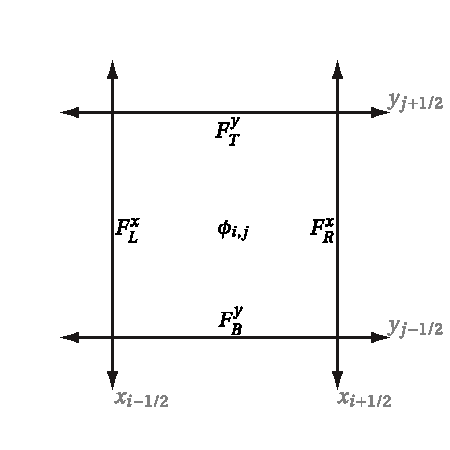
\includegraphics{cell-unknowns}
  \caption{Unknowns in cell $i,j$.}
  \label{fig:cellUnknowns}
\end{figure}

In all discretizations of the conservation equation, it is
essential that
$\vec{F}$ be continuous at cell interfaces: e.g., $F_T^y$ in cell~$i,j$ must
be equal to $-F_B^y$ in cell~$i,{j+1}$. Otherwise, the difference scheme is not
conservative.

\subsection{Anisotropic closure equations}

The radiation flux $\vec{F}$ and scalar intensity $\phi$ are related, in the
case of anisotropic diffusion, by the anisotropic Fick's law
of Eq.~\eqref{eq:adFicks}:
\begin{equation*}
  \vec{F}(\vec{x}) = - \Dtens(\vec{x}) \vd \grad \phi(\vec{x}) \,.
\end{equation*}
The anisotropic \Pone\ approximation, given in Eq.~\eqref{eq:ap1FicksLawFinal},
contains an additional term that accounts for stronger time dependence:
\begin{equation*}
  \frac{1}{c}\pder{\vec{F}}{t}(\vec{x},t)
  + \varsigma(\vec{x}) \Dtens(\vec{x}) \vd \grad \phi(\vec{x}, t)
  + \varsigma(\vec{x})\vec{F}(\vec{x},t) 
  = 0 \,.
\end{equation*}
We discretize this equation implicitly in time in accordance with the
semi-implicit approximation. Applying the backward Euler approximation to
$\phi$ and $\vec{F}$, then solving for $\vec{F}$, we obtain:
\begin{subequations}\label{eqs:ap1FicksImplicit}
\begin{equation}\label{eq:ap1FicksImplicit}
  \vec{F}(\vec{x}) = - [1 - \eta(\vec{x})]\Dtens(\vec{x}) \vd \grad \phi(\vec{x})
  + \eta(\vec{x}) \hat{\vec{F}}(\vec{x})\,,
\end{equation}
where $\vec{F}(\vec{x}) = \vec{F}(\vec{x}, t^{n+1})$,
$\hat{\vec{F}}(\vec{x})=\vec{F}(\vec{x}, t^n)$, and
\begin{equation}\label{eq:ap1ImplicitEta}
  \eta(\vec{x}) \equiv \frac{1}{1 + \varsigma(\vec{x}) c \Delta_t}\,.
\end{equation}
\end{subequations}
Setting $\eta=0$ reduces this equation to Eq.~\eqref{eq:adFicks2d}. (We will
use this fact to simplify the derivation of boundary conditions

%The finite difference schemes presented in this chapter approximate
%Eqs.~\eqref{eq:ap1FicksLawFinal} and~\eqref{eq:ap1FicksImplicit} on cell edges,
%while conserving energy, to relate the cell-averaged $\phi$ of adjacent cells.

Equation~\eqref{eq:ap1FicksImplicit} in 2-D comprises two equations in vector
form:
\begin{align}\label{eq:ficks2d}
  \begin{bmatrix}
    F^{x} \\
    F^{y}
  \end{bmatrix}
  &= - (1 - \eta)
  \begin{bmatrix}
    D^{xx} & D^{yx} \\
    D^{xy} & D^{yy}
  \end{bmatrix}
  \begin{bmatrix}
    \tpder{\phi}{x} \\
    \tpder{\phi}{y}
  \end{bmatrix}
  + \eta
  \begin{bmatrix}
    \hat{F}^{x} \\
    \hat{F}^{y}
  \end{bmatrix}
  \\ \nonumber
  &= 
  \begin{bmatrix}
    - (1 - \eta)D^{xx} \tpder{\phi}{x}
    - (1 - \eta)D^{yx} \tpder{\phi}{y}
    + \eta \hat{F}^{x}
    \\
    - (1 - \eta)D^{yy} \tpder{\phi}{y}
    - (1 - \eta)D^{xy} \tpder{\phi}{x}
    + \eta \hat{F}^{x}
  \end{bmatrix}
  \,.
\end{align}
The diagonal components of $\Dtens$ contribute to ``normal''
leakage; and the off-diagonal components $D^{xy}$ contribute to ``transverse''
leakage, particle movement \emph{across} the face due to a gradient
\emph{along} the face.
Note that since the anisotropic diffusion tensor is symmetric,
$D^{yx}=D^{xy}$.

Setting $\eta=0$ in Eq.~\eqref{eq:ficks2d} reduces the \APone\ equation to
the anisotropic Fick's law:
\begin{equation}\label{eq:adFicks2d}
  \begin{bmatrix}
    F^{x} \\
    F^{y}
  \end{bmatrix}
  = -
  \begin{bmatrix}
    D^{xx} & D^{yx} \\
    D^{xy} & D^{yy}
  \end{bmatrix}
  \begin{bmatrix}
    \tpder{\phi}{x} \\
    \tpder{\phi}{y}
  \end{bmatrix}
  = 
  \begin{bmatrix}
    - D^{xx} \tpder{\phi}{x}
    - D^{yx} \tpder{\phi}{y}
    \\
    - D^{yy} \tpder{\phi}{y}
    - D^{xy} \tpder{\phi}{x}
  \end{bmatrix}
  \,.
\end{equation}

The finite difference schemes presented in this chapter approximate these
equations for $F^{x}$ and $F^{y}$ on cell edges. These approximations are then
used to relate the cell-centered $\phi$ from the conservation
equation~\eqref{eq:ssConservation}.

%%%%%%%%%%%%%%%%%%%%%%%%%%%%%%%%%%%%%%%%%%%%%%%%%%%%%%%%%%%%%%%%%%%%%%%%%%%%%%%%
\section{Neglecting transverse diffusion}\label{sec:discreteDiag}

Under a simplifying assumption about the structure of the anisotropic diffusion
tensor, very simple existing centered difference schemes can be
applied to AD and \APone. The conservative cell-centered diffusion scheme is
derived in Ref.~\cite{Dud1976}; the \APone\ difference scheme is a minor
extension \cite{War2003}.

In the structured Cartesian geometry we consider, the simplifying assumption is
to neglect the off-diagonal terms of the diffusion tensor that cause transverse
leakage.
In certain simple problems, however, this is not an approximation. If the
opacity is invariant with respect to one of the Cartesian coordinate system's
axes (see \S\ref{sec:adVoids}), the off-diagonal terms of $\Dtens$ are
identically zero. For problems in which transverse leakage is non-negligible,
the discretization scheme in this chapter must be used with caution: it is not
truly consistent with the underlying mixed-derivative partial differential
equation. Even as the grid size approaches zero, the off-diagonal diffusion
components are still neglected.

The simple ``diagonal-only'' centered difference scheme is also useful as an
instructive tool, because we later develop a more complex difference scheme that
uses the same principles.

%%%%%%%%%%%%%%%%%%%%%%%%%%%%%%%%%%%%%%%%
\subsection{Anisotropic diffusion}
The discretization scheme for anisotropic diffusion presented here is only a
slight modification of common cell-centered diffusion scheme: the
orientation of the faces determines which component of the anisotropic diffusion
tensor is used.  This centered difference scheme was used in the earliest work
on the anisotropic diffusion approximation \cite{Lar2009c}.

Setting $D^{yx}=D^{xy}=0$ simplifies Eq.~\eqref{eq:adFicks2d} to:
\begin{equation*}
  \begin{bmatrix}
    F^{x} \\
    F^{y}
  \end{bmatrix}
  = -
  \begin{bmatrix}
    D^{xx} & 0 \\
    0 & D^{yy}
  \end{bmatrix}
  \begin{bmatrix}
    \tpder{\phi}{x} \\
    \tpder{\phi}{y}
  \end{bmatrix}
  = 
  \begin{bmatrix}
    - D^{xx} \tpder{\phi}{x} \\
    - D^{yy} \tpder{\phi}{y}
  \end{bmatrix}
  \,.
\end{equation*}

Without loss of generality, we evaluate the face-averaged flux from cell
$i,j$ through its right face, which has an outer normal along the $+x$ axis,
$\vec{n}_R = [1,0]$:
\begin{align} \nonumber
  F_R^x &\equiv \frac{1}{\Delta_{y,j}} \int_{y_{j-1/2}}^{y_{j+1/2}}
  \vec{F}(x_{i+1/2}, y) \vd \vec{n}_R \ud y\,.
  \\
  \intertext{Substituting the anisotropic Fick's law, we obtain} \nonumber
  F_R^x &= - \frac{1}{\Delta_{y,j}} \int_{y_{j-1/2}}^{y_{j+1/2}}
  D_{i,j}^{xx} \pder{\phi}{x} \ud y \,.
  \\ 
  \intertext{Now we introduce a temporary value $\phi_*$ on the edge of the cell
    to
  approximate the partial derivative using a second-order finite difference
  stencil:}
  \label{eq:diagFrx}
  F_R^x &\approx - 
  D_{i,j}^{xx} \frac{\phi_* - \phi_{i,j}}{\Delta_{x,i}/2} \,.
\end{align}
To be conservative, this term must be equal to $F_L^x$ from the cell to
the right. Evaluating the flux across the same face in the $+x$ direction
from the perspective of cell $i+1,j$, and approximating the derivative using the
same edge-centered $\phi_*$, we obtain
\begin{equation}\label{eq:diagFlx}
  F_{L,i+1,j}^x \approx - 
  D_{i+1,j}^{xx} \frac{\phi_{i+1,j} - \phi_*}{\Delta_{x,i+1}/2} \,.
\end{equation}
Scaling Eqs.~\eqref{eq:diagFrx} and~\eqref{eq:diagFlx} by $\Delta_x/(2 D^{xx})$
and adding them, we eliminate $\phi_*$:
\begin{equation*}
  \frac{\Delta_{x,i}/2}{D_{i,j}^{xx}}F_R^x
 + \frac{\Delta_{x,i+1}/2}{D_{i+1,j}^{xx}}F_{L,i+1,j}^x
 = \left[ -(\phi_* - \phi_{i}) \right] + \left[ -(\phi_{i+1,j} - \phi_*)
   \right]
   = -\left( \phi_{i+1,j} - \phi_{i,j} \right) \,.
\end{equation*}
We enforce particle conservation by setting $F_{L,i+1,j}^x = F_R^x$, and we
solve for $F_R^x$. This
gives the following expression for the net leakage through the right face of
cell $i,j$:
\begin{equation}\label{eq:diagF}
  F_R^x= -\frac{D^{xx}_{i+1/2,j}}{\Delta_{x,i+1/2}}
  \left( \phi_{i+1,j} - \phi_{i,j} \right)\,.
\end{equation}
Here we have defined a harmonically averaged cell-edge diffusion coefficient:
\begin{equation} \label{eq:cellEdgeDHarmonic}
  \frac{D^{xx}_{i+1/2,j}}{\Delta_{x,i+1/2}} \equiv \left[
  \frac12 \left( \frac{D^{xx}_{i,j}}{\Delta_{x,i}} \right)\inv
 + \frac12 \left( \frac{D^{xx}_{i+1,j}}{\Delta_{x,i+1}} \right)\inv
  \right]\inv\,.
\end{equation}
This is the standard relation between neighboring cells in the
cell-centered discretization scheme \cite{Dud1976}, except that in anisotropic
diffusion, leakage across the face normal to the $x$ axis takes the $D^{xx}$
component of the diffusion tensor.

The same procedure yields similar for the three other faces of cell $i,j$:
\begin{align*}
  F_L^x &= -\frac{D^{xx}_{i-1/2,j}}{\Delta_{x,i-1/2}}
  \left( \phi_{i,j} - \phi_{i-1,j} \right)\,,
  \\
  F_T^y &= -\frac{D^{yy}_{i,j+1/2}}{\Delta_{y,j+1/2}}
  \left( \phi_{i,j+1} - \phi_{i,j} \right)\,,
  \\
  F_B^y &= -\frac{D^{yy}_{i,j-1/2}}{\Delta_{y,j-1/2}}
  \left( \phi_{i,j} - \phi_{i,j-1} \right)\,.
\end{align*}
These terms, substituted into Eq.~\eqref{eq:ssConservationDisc}, relate the
cell-centered values of $\phi$ in the interior of the system:
\begin{multline} \label{eq:diagConservation}
  \hphantom{ {}+{} }
  \Delta_{x,i} \left(
  - \frac{D^{yy}_{i,j+1/2}}{\Delta_{y,j+1/2}} \left( \phi_{i,j+1} - \phi_{i,j}
    \right)
  + \frac{D^{yy}_{i,j-1/2}}{\Delta_{y,j-1/2}} \left( \phi_{i,j} - \phi_{i,j-1}
    \right)
  \right)
\\
\shoveleft{%
  {}+ \Delta_{y,j} \left(
  - \frac{D^{xx}_{i+1/2,j}}{\Delta_{x,i+1/2}} \left( \phi_{i+1,j} - \phi_{i,j}
    \right)
  + \frac{D^{xx}_{i-1/2,j}}{\Delta_{x,i-1/2}} \left( \phi_{i,j} - \phi_{i-1,j}
    \right)
  \right)
}
\\
{}+ \Delta_{x,i}\Delta_{y,j} \sigma_{a,i,j} \phi_{i,j}
= \Delta_{x,i}\Delta_{y,j} q_{i,j}\,.
\end{multline}
Rearranging shows the leakage terms to be part of a discretized Laplacian
operator. In fact, if $\Delta_x = \Delta_y = h$, and
$\Dtens(\vec{x})=D\Identitytens$, then Eq.~\eqref{eq:diagConservation} reduces
to a well-known five-point stencil:
\begin{equation*}
  -\frac{D}{h^2}\left( \phi_{i+1,j} + \phi_{i,j+1} + \phi_{i-1,j}
  + \phi_{i,j-1} - 4\phi_{i,j} \right) + \sigma_{a} = q\,.
\end{equation*}

When a cell has one or more faces on an exterior boundary, the above relations
for $\vec{n}\vd \vec{F}$ are replaced by a discretized form of the boundary
condition, which we shall derive presently.

%%%%%%%%%%%%%%%%%%%%%%%%%%%%%%%%%%%%%%%%
\subsection{Anisotropic \texorpdfstring{\Pone}{P1}}

The time-dependent \Pone\ and anisotropic \Pone\ methods have as unknowns the
radiation flux $\vec{F}$ in addition to the scalar intensity $\phi$. Using the
same finite differencing procedure as performed above for anisotropic diffusion,
we obtain a discretization for \APone\ that stores $\phi$ in cell centers and
$\vec{F}$ on cell edges.
%Because the locations of the cell edges are distinct
%from the cell centers, this is known as a ``staggered grid'' approximation
%\cite{War2003}.
In the steady-state case, the edge-centered $\vec{F}$ terms can be eliminated
algebraically, and this discretization reduces to the above anisotropic
diffusion discretization.

We evaluate the 2-D anisotropic \Pone\ equation~\eqref{eq:ficks2d} on the right
face of cell $i,j$, set $D^{yx}=0$, and introduce the temporary edge-centered
$\phi_*$ to approximate the derivative normal to the face:
\begin{equation*}
  F_{i+1/2,j}^{x} =
  - (1 - \eta_{i,j})D_{i,j}^{xx} \frac{\phi_* - \phi_{i,j}}{\Delta_{x,i}/2}
  + \eta_{i,j} \hat{F}_{i+1/2,j}^{x} \,.
\end{equation*}
Evaluating the leakage on same face from cell $i+1,j$, we obtain:
\begin{equation*}
  F_{i+1/2,j}^{x} =
  - (1 - \eta_{i+1,j})D_{i+1,j}^{xx} \frac{\phi_{i+1,j} - \phi_*}{\Delta_{x,i+1}/2}
  +  \eta_{i+1,j} \hat{F}_{i+1/2,j}^{x} \,.
\end{equation*}
Multiplying the equations by $(\Delta_{x} / 2) / [(1 - \eta) D^{xx}]$, we
eliminate the temporary $\phi_*$ to arrive at the following conservative
equation:
\begin{subequations}\label{eqs:diagApone}
\begin{multline}\label{eq:diagAponeX}
  \left[
    \frac{\Delta_{x,i}/2}{(1 - \eta_{i,j})D_{i,j}^{xx}}
  + \frac{\Delta_{x,i+1}/2}{(1 - \eta_{i+1,j})D_{i+1,j}^{xx}} \right]
  F_{i+1/2,j}^{x}
  \\ = \phi_{i,j} - \phi_{i+1,j}
  + \left[
    \frac{\eta_{i,j} \Delta_{x,i}/2}{(1 - \eta_{i,j})D_{i,j}^{xx}}
  + \frac{\eta_{i+1,j} \Delta_{x,i+1}/2}{(1 - \eta_{i+1,j})D_{i+1,j}^{xx}}
  \right] \hat{F}_{i+1/2,j}^{x}  \,.
\end{multline}

\thesisclearpage

For faces normal to the $y$ axis, the corresponding equation uses the $D^{yy}$
component of the diffusion tensor:
\begin{multline}\label{eq:diagAponeY}
  \left[
    \frac{\Delta_{y,j}/2}{(1 - \eta_{i,j})D_{i,j}^{yy}}
  + \frac{\Delta_{y,j+1}/2}{(1 - \eta_{i,j+1})D_{i,j+1}^{yy}} \right]
  F_{i,j+1/2}^{y}
  \\ = \phi_{i,j} - \phi_{i,j+1}
  + \left[
    \frac{\eta_{i,j} \Delta_{y,j}/2}{(1 - \eta_{i,j})D_{i,j}^{yy}}
  + \frac{\eta_{i,j+1} \Delta_{y,j+1}/2}{(1 - \eta_{i,j+1})D_{i,j+1}^{yy}}
  \right] \hat{F}_{i,j+1/2}^{y}  \,.
\end{multline}
\end{subequations}

Equations~\eqref{eqs:diagApone} relate the flux at a face with the scalar
intensity in the adjacent cells. They provide one equation for each interior
face; the conservation equation~\eqref{eq:ssConservationDisc} provides an
equation for each cell; and a discretization of the anisotropic \Pone\ boundary
conditions (described next) provides an equation for each boundary face.

%%%%%%%%%%%%%%%%%%%%%%%%%%%%%%%%%%%%%%%%%%%%%%%%%%%%%%%%%%%%%%%%%%%%%%%%%%%%%%%%
\subsection{Boundary conditions}\label{sec:discreteDiagBc}

The specified incident boundary condition for anisotropic diffusion is given in
Eq.~\eqref{eq:loBc}:
\begin{equation*}
2\int_{\vec{\Omega}\vd\vec{n} < 0} W(\abs{\vec{\Omega}\vd\vec{n}})
I^b \ud\Omega
=
\phi
+ 2 \vec{d} \vd \grad \phi\,,
\end{equation*}
where the transport-calculated boundary coefficient is given in
Eq.~\eqref{eq:adBoundaryIntegral}:
\begin{equation*}
  \vec{d} = -\int_{\vec{\Omega}\vd\vec{n} < 0} W(\abs{\vec{\Omega}\vd\vec{n}})
\vec{\Omega} f \ud\Omega\,.
\end{equation*}

The anisotropic \Pone\ boundary condition, Eq.~\eqref{eq:ap1BoundaryCondition},
is similar:
\begin{equation*}
  2 \int_{\vec{\Omega}\vd\vec{n} < 0}
  W(\abs{\vec{\Omega}\vd\vec{n}}) I^b \ud\Omega
  = \phi
  - 2 \vec{d} \vd \Dtens\inv \vd \vec{F} \,,
\end{equation*}
where $\vec{d}$ is the same as in anisotropic diffusion.
In fact, by substituting the time-discretized $\vec{F}$ from
Eq.~\eqref{eq:ap1FicksImplicit}, we obtain a general boundary condition that
reduces to the anisotropic diffusion boundary condition by setting $\eta=0$:
\begin{align*}
  2 \int_{\vec{\Omega}\vd\vec{n} < 0}
  W(\abs{\vec{\Omega}\vd\vec{n}}) I^b \ud\Omega
  &= \phi
  - 2 \vec{d} \vd \Dtens\inv \vd 
  \left[ - (1 - \eta)\Dtens \vd \grad \phi + \eta \hat{\vec{F}} \right]
  \\
  &=  \phi + 2 (1 - \eta) \vec{d} \vd \grad \phi
  - 2 \eta \vec{d} \vd \Dtens\inv \vd \hat{\vec{F}} \,.
\end{align*}

Looking ahead to using flatland geometry (Chapter~\ref{chap:flatland}) in
addition to standard 2-D geometry, we write this
AD/\APone\ boundary condition in a more general form:
\begin{equation}\label{eq:discreteBcGeneral}
  q = \phi + r (1 - \eta) \vec{d} \vd \grad \phi
  - r \eta \vec{d} \vd \Dtens\inv \vd \hat{\vec{F}}\,,
\end{equation}
where $q$, $r$, $\vec{d}$, and $\Dtens$ all depend upon the chosen geometry. The
values $q$ and $r$ are given in Table~\ref{tab:discreteBcCoeffs}.
%
\begin{table}[htb]
  \centering
  \begin{tabular}{rcc}
\toprule
& $q$
& $r$
\\ \midrule
1-D/2-D/3-D
& $2 \int_{\vec{\Omega}\vd\vec{n} < 0}
  W(\abs{\vec{\Omega}\vd\vec{n}}) I^b \ud\Omega$
  & $2\vphantom{\Big|}$
\\
Flatland
& $2 \pi \int_{\vec{\Omega}\vd\vec{n} < 0}
  V(\abs{\vec{\Omega}\vd\vec{n}}) I^b \ud\Omega$
& $\pi/2\vphantom{\Big|}$
\\ \bottomrule
  \end{tabular}
  \Caption{Coefficients for the discretized boundary conditions.}{
    The flatland values
    and the function $V$ are discussed in Chapter~\ref{chap:flatland}.}
  \label{tab:discreteBcCoeffs}
\end{table}

At this point, Eq.~\eqref{eq:discreteBcGeneral} applies to arbitrary geometries,
both anisotropic methods, and problems in which $D^{xy} \ne 0$.
Now we make the analysis slightly less general by demanding
that $\eta$ be azimuthally symmetric about the outward normal of the boundary face.
(Equivalently, we discard the $D^{yx}=D^{xy}$ terms if the boundary face is
along one of the coordinate axes.) With this assumption, as discussed in
\S\ref{sec:adLinalg}, the normal vector $\vec{n}$ of the boundary face is an
eigenvector of $\Dtens$:
\begin{equation*}
  \Dtens \to D \vec{n}\vec{n}\,,
\end{equation*}
and the boundary coefficient is pointed along the outward normal:
\begin{equation*}
  \vec{d} \to d \vec{n}\,.
\end{equation*}

Under this assumption, Eq.~\eqref{eq:discreteBcGeneral} simplifies
(using the fact that $\vec{n}$ is a unit vector):
\begin{align} \nonumber
  q &= \phi + r (1 - \eta) \left[ d \vec{n} \right] \vd \grad \phi
  - r \eta \left[ d \vec{n} \right] \vd \left[ D \vec{n}\vec{n} \right] \vd
  \hat{\vec{F}}\,,
  \\ \label{eq:discreteBcGeneralQ}
 q &=  \phi + (1 - \eta) dr \vec{n} \vd \grad \phi
  - \frac{\eta dr}{D} \hat{F} \,.
\end{align}
Here we have defined the outward component of the radiation flux at the
beginning of the time step ($t^n$):
\begin{equation*}
  \hat{F} \equiv  \vec{n} \vd \hat{\vec{F}} = \vec{n} \vd \vec{F}(t^n)\,.
\end{equation*}

In both the case of anisotropic diffusion and anisotropic \Pone, we seek the
exiting radiation flux on the boundary face, the dot
product of the outward normal $\vec{n}$ and Eq.~\eqref{eq:ap1FicksImplicit}:
\begin{align}\nonumber
  \vec{n} \vd\vec{F}
  &= - [1 - \eta]\vec{n} \vd \left[ D \vec{n} \vec{n}  \right] \vd \grad \phi
  + \eta \vec{n} \vd\hat{\vec{F}}
  \\ \label{eq:discreteBcGeneralF}
  F &= - [1 - \eta] D \vec{n} \vd \grad \phi + \eta \hat{F} \,,
\end{align}
where
\begin{equation*}
  F \equiv \vec{n} \vd \vec{F} \,.
\end{equation*}

Both Eqs.~\eqref{eq:discreteBcGeneralQ} and~\eqref{eq:discreteBcGeneralF}
are evaluated at the exterior boundary face.  In our discretization schemes, 
$F$ is located on the boundary, but $\phi$ is stored at cell centers.
To obtain a
boundary discretization accurate to $O(\Delta_x^2)$, we cannot approximate the
cell-edge value of $\phi$ with the cell-center value of $\phi$. Instead, we
introduce a temporary edge-centered $\phi_*$, approximating the directional
derivative in the two equations with:
\begin{equation*}
  \vec{n} \vd \grad \phi(\vec{x}_b) \approx \frac{\phi_* - \phi}{\Delta/2}\,,
\end{equation*}
where $\phi$ is the cell-centered scalar intensity, and $\Delta$ is the width of
the cell along direction normal to the boundary. Equations~\eqref{eq:discreteBcGeneralQ}
and~\eqref{eq:discreteBcGeneralF} then become:
\begin{subequations}\label{eqs:discreteBcGeneral2}
  \begin{align}\label{eq:discreteBcGeneralQ2}
 q &=  \phi + (1 - \eta) dr \frac{\phi_* - \phi}{\Delta/2}
  - \frac{\eta dr}{D} \hat{F} \,,
  \\ 
  \intertext{and} \label{eq:discreteBcGeneralF2}
  F &= - [1 - \eta] D\frac{\phi_* - \phi}{\Delta/2} + \eta \hat{F} \,.
  \end{align}
\end{subequations}
Eliminating $\phi_*$ in Eqs.~\eqref{eqs:discreteBcGeneral2},
we obtain an equation for the exiting
radiation flux on the boundary for the \APone approximation:
\begin{equation}\label{eq:discreteBcAponeFinal}
  F = \left[ \frac{\Delta/2}{1 - \eta} + dr \right]\inv
  \left[ D\phi - Dq - \eta dr \hat{F} \right]
  + \eta \hat{F} \,.
\end{equation}
Setting $\eta=0$ gives the discretized anisotropic diffusion boundary condition:
\begin{equation}\label{eq:discreteBcAdFinal}
  F = \left[ \Delta/2 + dr \right]\inv \left[ D\phi - Dq  \right] \,.
\end{equation}

If the 2-D Marshak approximation is used for the geometry and coefficients, then
$q=4F^-$, $r=2$, and $d=D$; and Eq.~\eqref{eq:discreteBcAdFinal} resultantly
reduces to the
discretized standard diffusion boundary condition:
\begin{equation*}
  F = \left[ \Delta/2 + 2D \right]\inv \left[ D\phi - 4DF^-  \right] \,.
\end{equation*}

%%%%%%%%%%%%%%%%%%%%%%%%%%%%%%%%%%%%%%%%%%%%%%%%%%%%%%%%%%%%%%%%%%%%%%%%%%%%%%%%
\section{Quasidiffusion-like discretization}

The discretization in \S\ref{sec:discreteDiag} relies on discarding the
components of the diffusion tensor that lead to transverse leakage. If those
components are non-negligible, i.e.~in a problem with opacities
that vary strongly along both the $x$ and $y$ axes, we would like a
more accurate discretization scheme that preserves those components.

One scheme is an adaptation an existing difference method for quasidiffusion
(QD) that is attributed to Fryazinov \cite{Fry1976}, used by Aksenov and Gol'din
\cite{Aks1979}, and implemented in several contemporary theses on the topic of
QD \cite{Val2002,Wie2009}. The discretization scheme is straightforward to
derive and implement using the following procedure:
\begin{enumerate}
  \item Let the unknown $\phi$ live at both the cell centers and the
  cell edges.%
  \footnote{%
  For an $M\times N$ Cartesian grid, this means $MN$
  cell-centered $\phi$ and $2MN + M + N$ edge-centered $\phi$, roughly treble
  the number of unknowns in the simple cell-centered difference scheme of
  \S\ref{sec:discreteDiag}.%
  }
  \item Integrate $\vec{F}\vd \vec{n}$ over half of a cell, approximating
  it as a constant in that domain.
  \item Use particle conservation to relate adjacent cells.
\end{enumerate}

Applying this procedure to anisotropic diffusion does not yield the same result
as given in Ref.~\cite{Val2002}. This is because, even though AD and QD both
contain tensors
in their approximations to the radiation flux, the placement of the gradient
operator $\grad$ differs. Steady-state AD uses the approximation
\begin{align*}
  \vec{F} &= - \Dtens \vd \grad \phi
  \\ 
  \intertext{whereas steady-state QD uses the approximation}
  \vec{F} &= - \frac{1}{\sigma} \grad \vd \Etens \phi\,.
\end{align*}

To apply the QD discretization to the anisotropic diffusion equation,
we integrate the Anisotropic Fick's law, Eq.~\eqref{eq:adFicks2d}, over the
right half of cell $i,j$ as represented in Fig.~\ref{fig:goldinRight}.

Integrating the anisotropic Fick's law, Eq.~\eqref{eq:adFicks2d}, over the right
half of cell $i,j$, as represented in Fig.~\ref{fig:goldinRight}, gives an
approximate expression for the flux exiting the right face $F_R^x =
\vec{F}\vd\vec{n}_R$:
\begin{align*}
\int_{y_{j-1/2}}^{y_{j+1/2}} \int_{x_{i}}^{x_{i+1/2}}
\vec{n}_R \vd \vec{F}
\ud x \ud y
&=
\int_{y_{j-1/2}}^{y_{j+1/2}} \int_{x_{i}}^{x_{i+1/2}}
-\vec{n}_R \vd \Dtens \vd \grad \phi
\ud x \ud y
\\
F_R^x \frac{\Delta_{x,i} \Delta_{y,j}}{2}
&=
-
\begin{bmatrix}
  1 & 0
\end{bmatrix}
\begin{bmatrix}
  D_{i,j}^{xx} & D_{i,j}^{yx} \\
  D_{i,j}^{xy} & D_{i,j}^{yy}
\end{bmatrix}
\int_{y_{j-1/2}}^{y_{j+1/2}} \int_{x_{i}}^{x_{i+1/2}}
\begin{bmatrix}
  \tpder{\phi}{x} \\
  \tpder{\phi}{y}
\end{bmatrix}
\ud x \ud y
\\
F_R^x \frac{\Delta_{x,i} \Delta_{y,j}}{2}
&=
-
\begin{bmatrix}
  D_{i,j}^{xx} & D_{i,j}^{yx}
\end{bmatrix}
\begin{bmatrix}
  \left( \phi_R - \phi_{i,j} \right) \Delta_{y,j} \\
  \left( \phi_T - \phi_B \right) \Delta_{x,i} / 2
\end{bmatrix}
\\
F_R^x
&= 
- D_{i,j}^{xx} \frac{\phi_R - \phi_{i,j}}{ \Delta_{x,i} / 2}
- D_{i,j}^{yx} \frac{\phi_T - \phi_B}{ \Delta_{y,j} }\ \,.
\end{align*}
%
\begin{figure}[htb]
  \centering
  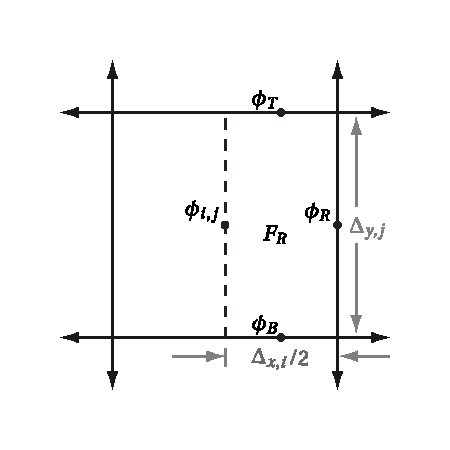
\includegraphics{goldin-righthalf}
  \caption{The right half of cell $i,j$.}
  \label{fig:goldinRight}
\end{figure}
%
Performing the same procedure for the left side, we obtain
\begin{align*}
\int_{y_{j-1/2}}^{y_{j+1/2}} \int_{x_{i-1/2}}^{x_{i}}
\vec{n}_L \vd \vec{F}
\ud x \ud y
&=
\int_{y_{j-1/2}}^{y_{j+1/2}} \int_{x_{i-1/2}}^{x_{i}}
-\vec{n}_L \vd \Dtens \vd \grad \phi
\ud x \ud y
\\
-F_L^x \frac{\Delta_{x,i} \Delta_{y,j}}{2}
&=
-
\begin{bmatrix}
  -1 & 0
\end{bmatrix}
\begin{bmatrix}
  D_{i,j}^{xx} & D_{i,j}^{yx} \\
  D_{i,j}^{xy} & D_{i,j}^{yy}
\end{bmatrix}
\int_{y_{j-1/2}}^{y_{j+1/2}} \int_{x_{i-1/2}}^{x_{i}}
\begin{bmatrix}
  \tpder{\phi}{x} \\
  \tpder{\phi}{y}
\end{bmatrix}
\ud x \ud y
\\
F_L^x \frac{\Delta_{x,i} \Delta_{y,j}}{2}
&=
-
\begin{bmatrix}
  D_{i,j}^{xx} & D_{i,j}^{yx}
\end{bmatrix}
\begin{bmatrix}
  \left( \phi_{i,j} - \phi_L \right) \Delta_{y,j} \\
  \left( \phi_T - \phi_B \right) \Delta_{x,i} / 2
\end{bmatrix}
\ud x \ud y
\\
F_L^x
&= 
- D_{i,j}^{xx} \frac{\phi_{i,j} - \phi_L}{ \Delta_{x,i} / 2}
- D_{i,j}^{yx} \frac{\phi_T - \phi_B}{ \Delta_{y,j} }\,.
\end{align*}

Rotating the coordinate system by swapping $x\leftrightarrow y$, $T
\leftrightarrow R$, $B \leftrightarrow L$, and $i \leftrightarrow j$, we obtain
analogous equations for the top and bottom leakage terms:
\begin{align*}
F_T^y
&= 
- D_{i,j}^{yy} \frac{\phi_T - \phi_{i,j}}{ \Delta_{y,j} / 2}
- D_{i,j}^{xy} \frac{\phi_R - \phi_L}{ \Delta_{x,i} }\,,
\\  
F_B^y
&= 
- D_{i,j}^{yy} \frac{\phi_{i,j} - \phi_B}{ \Delta_{y,j} / 2}
- D_{i,j}^{xy} \frac{\phi_R - \phi_L}{ \Delta_{x,i} }\,.
\end{align*}

At each interior face, we demand that the scalar intensity $\phi$ be continuous,
i.e.,
\begin{equation*}
  \phi_{R,i,j} = \phi_{L,i+1,j} \equiv \phi_{i+1/2,j}\,.
\end{equation*}
Substituting these definitions and the net leakage expressions into the
conservation equation~\eqref{eq:ssConservationDisc}, we obtain:
\begin{multline*}
- \Delta_{x,i} D_{i,j}^{yy}\frac{\phi_{i,j+1/2} - \phi_{i,j}}{\Delta_{y,j} / 2}
- \Delta_{x,i} D_{i,j}^{xy}\frac{\phi_{i+1/2,j} - \phi_{i-1/2,j}}{\Delta_{x,i} }
+ \Delta_{x,i} D_{i,j}^{yy}\frac{\phi_{i,j} - \phi_{i,j-1/2}}{\Delta_{y,j} / 2}
\\
\shoveleft{%
+ \Delta_{x,i} D_{i,j}^{xy}\frac{\phi_{i+1/2,j} - \phi_{i-1/2,j}}{\Delta_{x,i} }
- \Delta_{y,j} D_{i,j}^{xx}\frac{\phi_{i+1/2,j} - \phi_{i,j}}{\Delta_{x,i} / 2}
- \Delta_{y,j} D_{i,j}^{yx}\frac{\phi_{i,j+1/2} - \phi_{i,j-1/2}}{\Delta_{y,j} }
}
\\
+ \Delta_{y,j} D_{i,j}^{xx}\frac{\phi_{i,j} - \phi_{i-1/2,j}}{\Delta_{x,i} / 2}
+ \Delta_{y,j} D_{i,j}^{yx}\frac{\phi_{i,j+1/2} - \phi_{i,j-1/2}}{\Delta_{y,j} }
+ \Delta_{x,i}\Delta_{y,j} \sigma_{a,i,j} \phi_{i,j}
= \Delta_{x,i}\Delta_{y,j} q_{i,j}\,.
\end{multline*}
\begin{subequations}\label{eqs:goldin}
The transverse leakage terms cancel, leaving a conservative relation between the
cell-centered $\phi_{i,j}$ and the surrounding edge-centered $\phi$:
\begin{multline}\label{eq:goldinCenter}
\phi_{i,j} \left(
   4 D_{i,j}^{xx} \frac{\Delta_{y,j}}{\Delta_{x,i}}
 + 4 D_{i,j}^{yy} \frac{\Delta_{x,i}}{\Delta_{y,j}}
 + \Delta_{x,i}\Delta_{y,j} \sigma_{a,i,j} \right)
 \\
- 2 D_{i,j}^{xx} \frac{\Delta_{y,j}}{\Delta_{x,i}}
  \left( \phi_{i+1/2,j} + \phi_{i-1/2,j} \right)
- 2 D_{i,j}^{yy} \frac{\Delta_{x,i}}{\Delta_{y,j}}
  \left( \phi_{i,j+1/2} + \phi_{i,j-1/2} \right)
\\= \Delta_{x,i}\Delta_{y,j} q_{i,j}\,.
\end{multline}

To complete the equations for the QD-like discretization, we enforce continuity
of the radiation flux on interior faces. On the top face, we set $F_{T,i,j}^y =
F_{B,i,j+1}^y$ to obtain equations for horizontal cell edges in the interior:
\begin{multline}\label{eq:goldinEdgeY}
- D_{i,j}^{yy} \frac{\phi_{i,j+1/2} - \phi_{i,j}}{ \Delta_{y,j} / 2}
- D_{i,j}^{xy} \frac{\phi_{i+1/2,j} - \phi_{i-1/2,j}}{ \Delta_{x,i} }
\\
=
- D_{i,j+1}^{yy} \frac{\phi_{i,j+1} - \phi_{i,j+1/2}}{ \Delta_{y,j} / 2}
- D_{i,j+1}^{xy} \frac{\phi_{i+1/2,j+1} - \phi_{i-1/2,j+1}}{ \Delta_{x,i} }\,.
\end{multline}
Setting $F_{R,i,j}^x = F_{L,i+1,j}^x$ yields equations for the interior vertical
edges:
\begin{multline}\label{eq:goldinEdgeX}
- D_{i,j}^{xx} \frac{\phi_{i+1/2,j} - \phi_{i,j}}{ \Delta_{x,i} / 2}
- D_{i,j}^{yx} \frac{\phi_{i,j+1/2} - \phi_{i,j-1/2}}{ \Delta_{y,j} }
\\
=
- D_{i+1,j}^{xx} \frac{\phi_{i+1,j} - \phi_{i,j}}{ \Delta_{x,i} / 2}
- D_{i+1,j}^{yx} \frac{\phi_{i+1,j+1/2} - \phi_{i+1,j-1/2}}{ \Delta_{y,j} }\,.
\end{multline}
\end{subequations}

If $D^{xy} = D^{yx}=0$, the edge-centered $\phi$ can be algebraically eliminated
without approximation, and
the QD-like method reduces to the simple cell-centered difference scheme of
\S\ref{sec:discreteDiag}.

Equations~\eqref{eqs:goldin} give one relation for each cell and interior edge.
The boundary conditions for this discretization are simpler to derive than those
in \S\ref{sec:discreteDiag}: because the edge-centered $\phi$ are actual
unknowns, there is no need to solve for $F$ and algebraically eliminate the edge
values in Eqs.~\eqref{eqs:discreteBcGeneral2}.
Only Eq.~\eqref{eq:discreteBcGeneralQ} by itself is necessary.

The greater number of unknowns inherent to this discretization are undesirable.
However, unlike the ``diagonal-only'' discretization from
\S\ref{sec:discreteDiag}, it does not make any approximations to the transverse
leakage terms. We have used this Gol'din discretization in our internal testing
to verify the discretizations presented in the next section, but we will not
use it in our final numerical experiments.

%%%%%%%%%%%%%%%%%%%%%%%%%%%%%%%%%%%%%%%%%%%%%%%%%%%%%%%%%%%%%%%%%%%%%%%%%%%%%%%%
\section{Nine-point stencil}

Because the QD-like method uses three times as many unknowns as the simple
cell-centered difference method given in \S\ref{sec:discreteDiag}, it is
computationally more expensive to solve. We desire a discretization scheme that
incorporates transverse leakage but has only $MN$ unknowns on an $M\times N$
structured Cartesian mesh. One way is to develop a stencil in which the
transverse
leakage is approximated using both the adjacent cell and cells along the
diagonal, as depicted in Fig.~\ref{fig:anisoStencils}.

\begin{figure}[b]
  \centering
  \subfloat[Transverse terms neglected]{%
  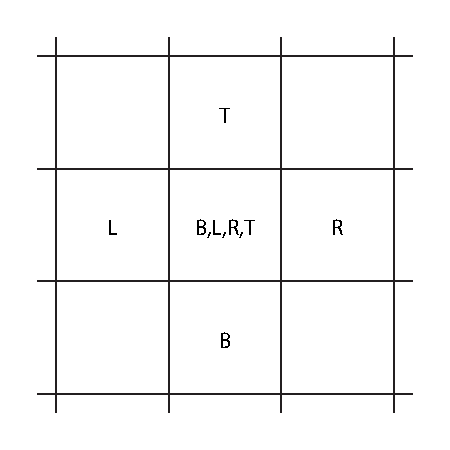
\includegraphics{diaganiso-leakage-terms}}
  \subfloat[Nine-point stencil]{%
  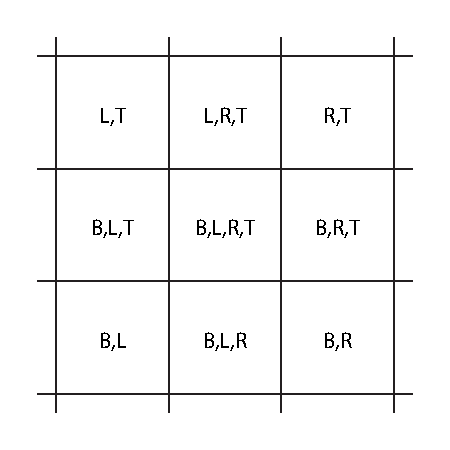
\includegraphics{cellaniso-leakage-terms}}
  \Caption{Stencils for $- \grad \vd \Dtens \grad \phi$.}{
  The leakage from each face $B,L,R,T$ depends on the
  values of $\phi$ in each cell with the corresponding letter.}
  \label{fig:anisoStencils}
\end{figure}

We begin by evaluating the face-averaged normal component of the flux,
$F_{i+1/2,j}^x \equiv \int_{y_{j-1/2}}^{y_{j+1/2}} \vec{F} \vd \vec{n} \ud
y$. We approximate the derivative normal
to the face by introducing an edge-centered $\phi_*$, using the same second-order
difference as in \S\ref{sec:discreteDiag}, and demanding that $F_{i+1/2,j}^x$ be
the same when from both cell $i,j$ and cell $i+1,j$.
Solving for $F_{i+1/2,j}^x$ gives a more general version of
Eq.~\eqref{eq:diagF}:
\begin{equation} \label{eq:cellAnisoFlux}
  F_{i+1/2,j}^{x} \approx
  - \frac{D^{xx}_{i+1/2,j}}{\Delta_{x,i+1/2}}
  \left[ 
    \left( \phi_{i+1,j} - \phi_{i,j} \right)
  + \frac{D^{xy}_{i,j}/D^{xx}_{i,j}}{2/\Delta_{x,i}}
    \pder{\phi}{y} \Bigg|_{x_{i+1/2}^-}
  + \frac{D^{xy}_{i+1,j}/D^{xx}_{i+1,j}}{2/\Delta_{x,i+1}}
    \pder{\phi}{y} \Bigg|_{x_{i+1/2}^+}
  \right]\,,
\end{equation}
where $\tpder{\phi}{y} |_{x_{i+1/2}^-}$ is the transverse derivative of
$\phi$ on the left side of the face, and $\tpder{\phi}{y} |_{x_{i+1/2}^+}$ is
the transverse derivative as viewed from the right side of the face.
The harmonically averaged diffusion coefficient is the same as in
Eq.~\eqref{eq:cellEdgeDHarmonic}:
\begin{equation*}
  \frac{D^{xx}_{i+1/2,j}}{\Delta_{x,i+1/2}} \equiv \left[
  \frac12 \left( \frac{D^{xx}_{i,j}}{\Delta_{x,i}} \right)\inv
 + \frac12 \left( \frac{D^{xx}_{i+1,j}}{\Delta_{x,i+1}} \right)\inv
  \right]\inv\,.
\end{equation*}

Figure~\ref{fig:cellAnisoLeakage} shows the net leakage from cell $i,j$ through
the
right face, and the surrounding cell-centered unknowns. Our goal is to
approximate Eq.~\eqref{eq:cellAnisoFlux} using only these cell-centered values,
without introducing extra unknowns.
%
\begin{figure}[htb]
  \centering
  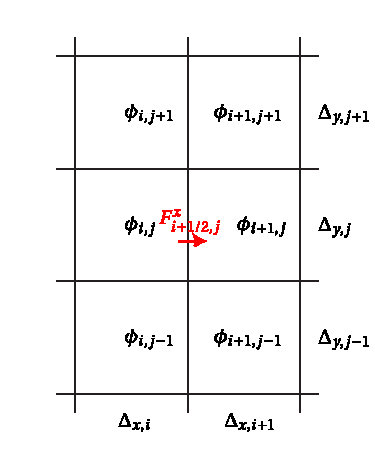
\includegraphics{cell-leakage-right}
  \caption{Diagram showing the radiation exiting interior cell $i,j$ through the
  right face.}
  \label{fig:cellAnisoLeakage}
\end{figure}

%%%%%%%%%%%%%%%%%%%%%%%%%%%%%%%%%%%%%%%%
\subsection{Stencil A}\label{sec:cellAnisoA}

One approximation to the transverse derivative in Eq.~\eqref{eq:cellAnisoFlux}
is the following second-order-accurate centered difference:
\begin{subequations}\label{eqs:cellAnisoA}
\begin{equation}\label{eq:cellAnisoA1}
  \pder{\phi}{y} \Bigg|_{x_{i+1/2}^-} \approx \frac{\phi_{i,j+1} -
  \phi_{i,j-1}}{\tfrac12 \Delta_{y,j+1} + \Delta_{y,j} + \tfrac12
  \Delta_{y,j-1}} \,.
\end{equation}
The transverse derivative on the right-hand side of the face is:
\begin{equation}\label{eq:cellAnisoA2}
  \pder{\phi}{y} \Bigg|_{x_{i+1/2}^+} \approx \frac{\phi_{i+1,j+1} -
  \phi_{i+1,j-1}}{\tfrac12 \Delta_{y,j+1} + \Delta_{y,j} + \tfrac12
  \Delta_{y,j-1}} \,.
\end{equation}
\end{subequations}

When cell $i,j$ is adjacent to the boundary in the transverse direction, we use
a backward difference stencil, given here in the case of evaluating the
transverse
leakage on the right face of cell $i,j$ when it is on the top boundary:
\begin{equation*}
  \pder{\phi}{y} \Bigg|_{x_{i+1/2}^-} \approx \frac{\phi_{i,j} -
  \phi_{i,j-1}}{\tfrac12 \Delta_{y,j} + \tfrac12 \Delta_{y,j-1}} \,.
\end{equation*}
Though this stencil is only first-order accurate, it avoids the severe
implementation penalty of involving the boundary conditions in the transverse
direction.\footnote{%
If second-order accuracy for the transverse leakage on the boundary is
\emph{truly} needed, an effective alternative to direct boundary conditions
might be the method of ``ghost cells.''}
If the cells adjacent to the boundary have no transverse leakage, this term is
not used. (Indeed, the boundary conditions derived in
\S\ref{sec:discreteDiagBc} require that assumption.)

%%%%%%%%%%%%%%%%%%%%%%%%%%%%%%%%%%%%%%%%
\subsection{Stencil B}

A different approximation to the transverse derivatives in
Eq.~\eqref{eq:cellAnisoFlux} is to formulate some to-be-determined approximate
edge centered $\phi$:
\begin{subequations}\label{eqs:cellAnisoB}
\begin{equation}\label{eq:cellAnisoPderY}
  \pder{\phi}{y} \Bigg|_{x_{i+1/2}^-} \approx \frac{\phi_{i,j+1/2} -
  \phi_{i,j-1/2}}{\Delta_{y,j}} \,,
\end{equation}
and
\begin{equation}\label{eq:cellAnisoPderY2}
  \pder{\phi}{y} \Bigg|_{x_{i+1/2}^+} \approx \frac{\phi_{i+1,j+1/2} -
  \phi_{i+1,j-1/2}}{\Delta_{y,j}} \,,
\end{equation}
or if the cell is not in the interior,
\begin{equation}\label{eq:cellAnisoPderY3}
  \pder{\phi}{y} \Bigg|_{x_{i+1/2}^-} \approx \frac{\phi_{i,j} -
  \phi_{i,j-1/2}}{\tfrac12 \Delta_{y,j} }\,.
\end{equation}
\end{subequations}

To derive an expression for $\phi_{i+1,j+1/2}$ that depends only on cells local
to $i,j$, we consider the finite difference scheme of \S\ref{sec:discreteDiag},
in which we introduced a temporary cell-edge unknown and discarded the off-diagonal
terms of the diffusion tensor. In evaluating Eq.~\eqref{eq:cellAnisoPderY} for
the transverse partial derivative in the $y$ direction, let us apply the
difference using conservation of energy, and discarding the transverse leakage
terms of this secondary equation.

The finite difference approximations coupling cell $i,j\equiv B$
to cell $i,j+1\equiv T$ via leakage through the top face, $F_{i,j+1/2} \equiv
F$ are:
\begin{equation*}
  F = - D_B \frac{\phi_* - \phi_B}{\Delta_B/2}
  \qquad\text{and}\qquad
  F = - D_T \frac{\phi_T - \phi_*}{\Delta_T/2}\,,
\end{equation*}
where $\phi_* \equiv \phi_{i+1,j+1/2}$. Before, we sought to eliminate
$\phi_*$. Now we wish to solve for it as an approximation to insert into
Eq.~\eqref{eq:cellAnisoPderY}, which is then used in
Eq.~\eqref{eq:cellAnisoFlux}.

Multiplying the equation for the bottom face by $\Delta_B / D_B$ and for the top
face by
$\Delta_T / D_T$, we obtain two equations:
\begin{equation*}
  -\frac{\Delta_B/2}{D_B } F = \phi_* - \phi_B
  \qquad\text{and}\qquad
  -\frac{\Delta_T/2}{D_T } F = \phi_T - \phi_* \,.
\end{equation*}
Adding them eliminates gives the standard finite-difference approximation for
$F$, seen in \S\ref{sec:discreteDiag}:
\begin{equation*}
  F = - \left( \frac{\Delta_B/2}{D_B } + \frac{\Delta_T/2}{D_T } \right)\inv
  \left( \phi_T - \phi_B \right),
\end{equation*}
and subtracting the second from the first gives an equation from which to solve
for $\phi_*$:
\begin{equation*}
 -\frac{\Delta_B/2}{D_B }F + \frac{\Delta_T/2}{D_T } F
 = 2 \phi_*-(\phi_B+\phi_T)\,.
\end{equation*}

Solving these two equations for $\phi_*$, we obtain the following expression:
\begin{equation}\label{eq:cellAnisoEdge}
  \phi_* = \frac{\Delta_B/D_B}{\Delta_T/D_T + \Delta_B/D_B} \phi_T
+ \frac{\Delta_T/D_T}{\Delta_T/D_T + \Delta_B/D_B} \phi_B \,.
\end{equation}
This equation approximates the cell-edge $\phi$ in the transverse direction as:
\begin{equation*}
  \phi_{i,j+1/2} \approx
  \frac{D_{i,j}^{yy} / \Delta_{y,j}}{D_{i,j+1}^{yy} / \Delta_{y,j+1} +
  D_{i,j}^{yy} / \Delta_{y,j}} \phi_{i,j+1}
+ \frac{D_{i,j+1}^{yy} / \Delta_{y,j+1}}{D_{i,j+1}^{yy} / \Delta_{y,j+1} +
D_{i,j}^{yy} / \Delta_{y,j}} \phi_{i,j} \,,
\end{equation*}
and
\begin{equation*}
  \phi_{i,j-1/2} \approx
  \frac{D_{i,j-1}^{yy} / \Delta_{y,j-1}}{D_{i,j}^{yy} / \Delta_{y,j} +
  D_{i,j-1}^{yy} / \Delta_{y,j-1}} \phi_{i,j}
+ \frac{D_{i,j}^{yy} / \Delta_{y,j}}{D_{i,j}^{yy} / \Delta_{y,j} +
D_{i,j-1}^{yy} / \Delta_{y,j-1}} \phi_{i,j-1} \,.
\end{equation*}
These edge values are then introduced into Eqs.~\eqref{eqs:cellAnisoB} to
approximate the transverse leakage through a face normal to the $x$ axis. In
the interior, then,
\begin{align*}
  \pder{\phi}{y} \Bigg|_{x_{i+1/2}^-} & \approx
  \frac{\phi_{i,j+1/2} - \phi_{i,j-1/2}}{\Delta_{y,j}}
  \\
  &= \frac{1}{\Delta_{y,j}} \Bigg[
  \frac{D_{i,j}^{yy} / \Delta_{y,j}}{D_{i,j+1}^{yy} / \Delta_{y,j+1} +
  D_{i,j}^{yy} / \Delta_{y,j}} \phi_{i,j+1}
+ \frac{D_{i,j+1}^{yy} / \Delta_{y,j+1}}{D_{i,j+1}^{yy} / \Delta_{y,j+1} +
D_{i,j}^{yy} / \Delta_{y,j}} \phi_{i,j}
\\
&\qquad\qquad -
  \frac{D_{i,j-1}^{yy} / \Delta_{y,j-1}}{D_{i,j}^{yy} / \Delta_{y,j} +
  D_{i,j-1}^{yy} / \Delta_{y,j-1}} \phi_{i,j}
- \frac{D_{i,j}^{yy} / \Delta_{y,j}}{D_{i,j}^{yy} / \Delta_{y,j} +
D_{i,j-1}^{yy} / \Delta_{y,j-1}} \phi_{i,j-1}
    \Bigg] \,.
\end{align*}


If the anisotropic diffusion coefficients are homogeneous and the grid is
uniform, Eq.~\eqref{eq:cellAnisoEdge} and Eqs.~\eqref{eqs:cellAnisoB} simplify
to Eqs.~\eqref{eqs:cellAnisoA}. The nine-point stencil for $-\grad \vd \grad
\phi$ becomes:
\begin{alignat*}{3}
  \tfrac{1}{2}D^{xy} & \phi_{i-1,j+1} \quad&
             -D^{yy} & \phi_{i,j+1} \quad&
 -\tfrac{1}{2}D^{xy} & \phi_{i+1,j+1}\quad
\\
             -D^{yy} & \phi_{i-1,j} &
 +\left( 2D^{xx} + 2D^{yy} \right) & \phi_{i,j} &
             -D^{xx} & \phi_{i+1,j}
\\
 -\tfrac{1}{2}D^{xy} & \phi_{i-1,j-1} &
             -D^{yy} & \phi_{i,j-1} \quad&
  +\tfrac{1}{2}D^{xy} & \phi_{i+1,j-1} \,.
\end{alignat*}

%%%%%%%%%%%%%%%%%%%%%%%%%%%%%%%%%%%%%%%%%%%%%%%%%%%%%%%%%%%%%%%%%%%%%%%%%%%%%%%%
\section{Summary}

We have derived several discretizations of the anisotropic diffusion and
anisotropic \Pone\ equations. The first simple discretization, in which
transverse
leakage is neglected, is a minor modification of existing cell-centered
difference schemes. The second quasi-diffusion-like scheme is a new application
of an existing methodology, but it undesirably introduces additional unknowns.
(We have used this scheme internally to compare against other discretizations,
but we will not employ it further.)
The final discretization scheme is, as far as we are aware, a novel extension of
standard cell differencing. It accounts for the ``transverse leakage''
introduced by the off-diagonal components of the diffusion tensor, yet it
retains the compact unknown space of simple cell-centered finite difference
methods.

